\section{New Hardware @ Mainz}
\begin{frame}{New hardware at Mainz}{}
	\begin{block}{High performance 12-core PC Dell R710}
		Two X5670 CPUs (24 virtual CPUs) @ 2.93GHz (3.33GHz turbo) \\
		24GB memory @ 1333MHz\\
		6*500GB with a fast PERC H700 ($\approx 450\frac{MB}{s}$ serial writing)\\
		Special ATLAS conditions: 3500€ 			
	\end{block}
	
	\begin{block}{Low power 12-core PC Dell R710}
		Two L5640 CPUs (24 virtual CPUs) @ 2.26GHz (2.8GHz turbo)\\
		24GB memory @ 1333MHz\\
		6*500GB with a fast PERC H700 ($\approx 450\frac{MB}{s}$ serial writing)\\
		Special ATLAS conditions: 3200€ 			
	\end{block}

	\begin{block}{48 x 1G-port switch Dell PowerConnect 6248}
		two SFP+ modules (two ports each)\\
		Special ATLAS conditions: 888€ + 100€ 
	\end{block}
\end{frame}

\begin{frame}{New hardware at Mainz}{}
	\begin{center} 
		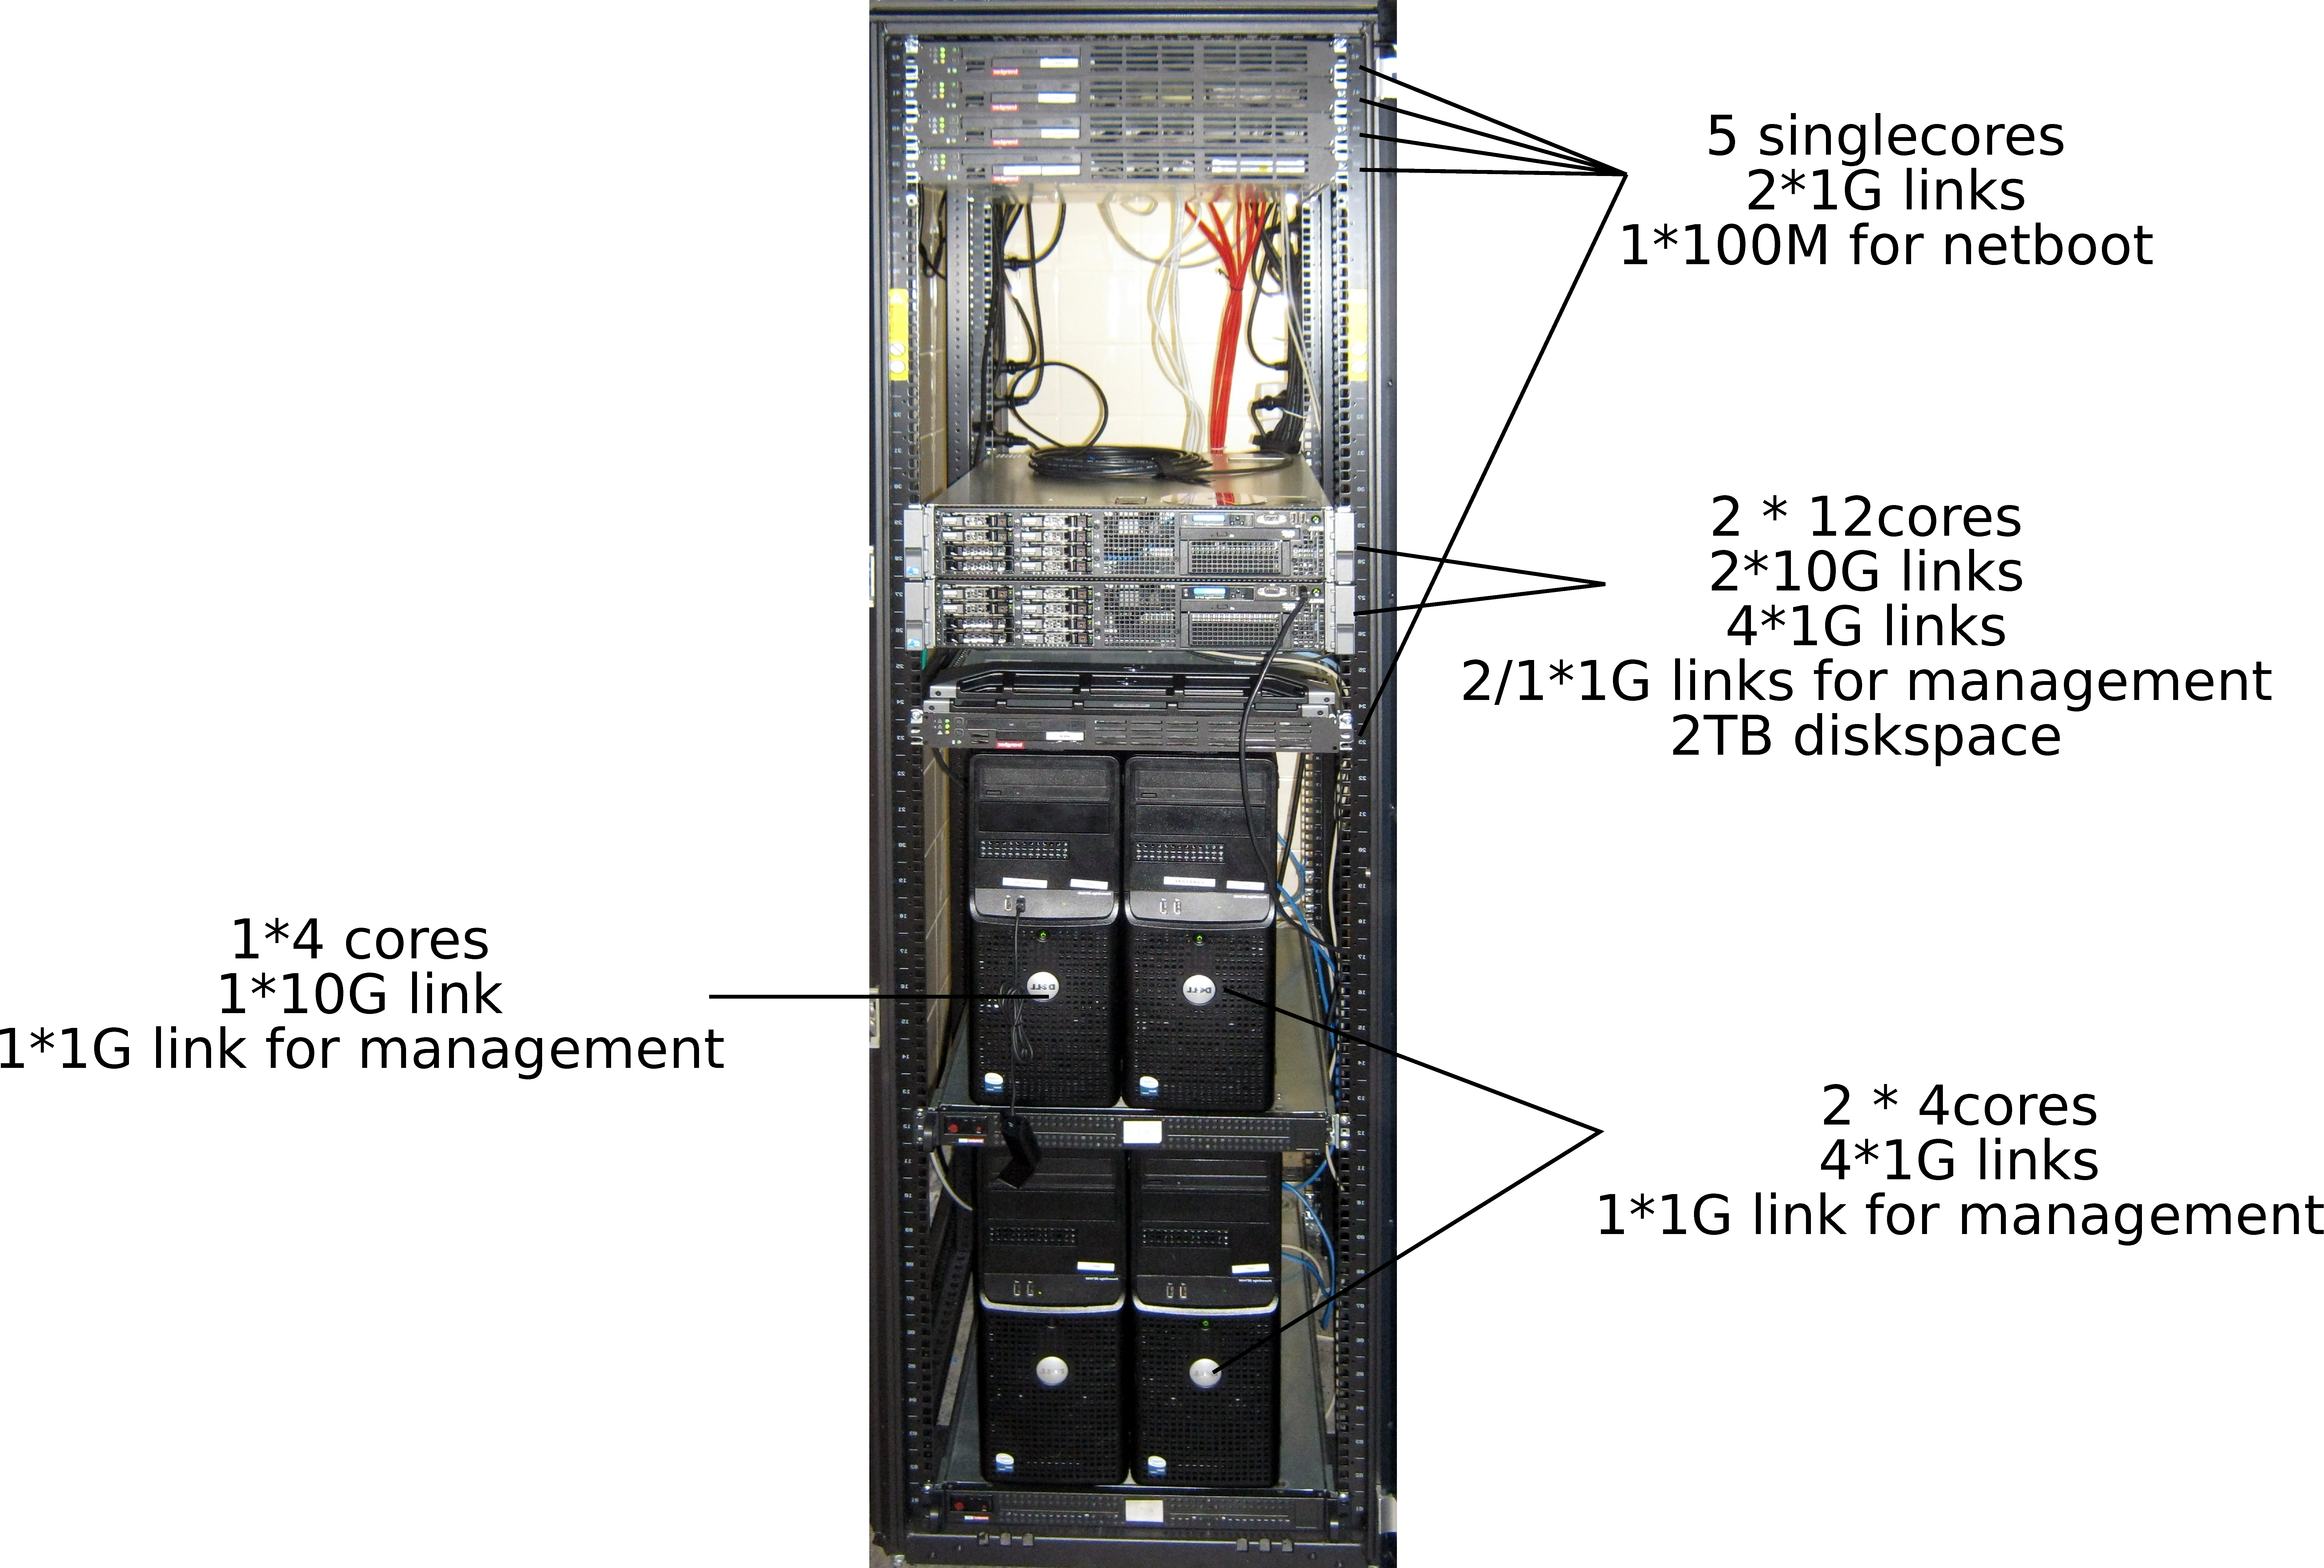
\includegraphics[height=7cm]{rack-overview}
	\end{center} 
\end{frame}

\begin{frame}{Power consumption with different power supplies}{}
	\begin{table}
	\begin{tabular}{lllll} 
	Power supply:	&	1x570 	&	2x570 	& 1x870	&	2x870\\ 
	\hline 
	low load	&	$156 \pm 3$		& $163 \pm 3$		& $171 \pm 3$	& \textbf{190}$ \pm 4$\\ 
	high load	&	$324 \pm 6$		& $332 \pm 7$		& $329 \pm 6$	& \textbf{351}$ \pm	7$
	\end{tabular} 
	\caption{Power consumption of the high performance PC in Watts}
	\end{table}	
	\begin{table}
	\begin{tabular}{lllll}
	Power supply:	&	1x570 	&	2x570 	& 1x870	&	2x870\\
	\hline
	low	load	&	$101 \pm 2$		& \textbf{113}$ \pm 2$		& $114 \pm 2$	& $138 \pm 2$ \\
	high load	&	$249 \pm 4$		& \textbf{252}$ \pm 4$		& $250 \pm 4$	& $273 \pm 4$
	\end{tabular}
	\caption{Power consumption of the low power PC in Watts}
	\end{table}
	High load via linpack (10k equations) benchmarks (HT on) taking 19GB memory:\\
	% messung hier mit nur einem prozess-> power unabh von oben:
	Fast PC: 102 GFLOPS (\textbf{292} $\frac{MFLOPS}{Watt}$) \\ 
	Low Power PC: 82 GFLOPS (\textbf{337} $\frac{MFLOPS}{Watt}$)
\end{frame}

\begin{frame}{Let's talk about racks}{}
	\begin{block}{10kW racks are suggested so far}
		351 Watts per PC $\Rightarrow$ up to 28 PCs per rack \\
		\begin{ergo}
			2U-PCs fit without a problem!
		\end{ergo}
	\end{block}
	If you really want to buy expensive 2U-PCs I would put disks into every PC
	instead of building a separate disk farm (Dell R510: up to 12 x 3,5" disks per
	PC) $\rightarrow$ need 100PCs to achieve 300TB. 
\\
	Better: Buy 1U-PCs and external raid arrays! (also if you want a separate farm) 
	
\end{frame}


\section{TCP: more than just reliable transmission}

\begin{frame}{Flow control}{Sliding window}
	\begin{center} 
	\includegraphics[height=0.7\textheight]{dataflowWindowSize}
	\end{center} 
\end{frame}

\begin{frame}{Congestion Avoidance}{Congestion window}
	\begin{center} 
		\includegraphics[width=0.8\textwidth]{slowStartundCongestionAvoidance}
	\end{center} 
\end{frame}

\section{Performance tests}

\begin{frame}{Packet sizes}{}
	\begin{center}
	  \includegraphics[width=0.97\textwidth]{udp-tcp-1048576-direct}
	\end{center}
\end{frame}

\begin{frame}{Interrupt coalescence}{Data rate}
	1$\mu s \hat{=}$ automatic calibration of interrupt coalescence
	\begin{center} 
	\includegraphics[height=0.53\textheight]{24threads-direct_2097152_udp-heat}
	\includegraphics[height=0.53\textheight]{24threads-direct_2097152_tcp-heat}
	\end{center} 
\end{frame}
\begin{frame}{Interrupt Coalescence}{CPU load}
	1$\mu s \hat{=}$ automatic calibration of interrupt coalescence
	\begin{center} 
	\includegraphics[height=0.53\textheight]{cpu24threads-switch_2097152_udp-heat}
	\includegraphics[height=0.53\textheight]{cpu24threads-switch_2097152_tcp-heat}
	\end{center} 
\end{frame}

\begin{frame}{Window sizes}{}
	I've run several tests with different memory settings and a interrupt
	coalescence of $1\mu s$:
	\begin{block}{Settings}
		sysctl -w "net.ipv4.tcp\_rmem=\$i \$i \$i" \\
		sysctl -w "net.ipv4.tcp\_wmem=\$i \$i \$i"\\
		sysctl -w "net.core.rmem\_max=\$i"\\
		sysctl -w "net.core.wmem\_max=\$i"\\
		sysctl -w "net.ipv4.udp\_mem=\$i \$i \$i"\\
		sysctl -w "net.ipv4.udp\_rmem\_min=\$i"\\
		sysctl -w "net.ipv4.udp\_wmem\_min=\$i"
	\end{block}
\end{frame}

\begin{frame}{Window sizes}{}
	\begin{center} 
	\includegraphics[height=0.53\textheight]{24threads-direct-mem-udp}
	\includegraphics[height=0.53\textheight]{24threads-direct-mem-tcp}
	\end{center} 
	The second bin is the default value
\end{frame}

\begin{frame}{Conclusions}{}
We should use TCP because:
\begin{itemize}
  \item Flow control and congestion avoidance
  \item TCP-optimized hardware (offload etc.)
  \item Adding reliability on top of UDP only in user mode (TCP: inside Kernel)!
  \item UDP: can only write MTU to socket; TCP: data stream instead
  \item Naggle algorithm helps you sending large packages (low CPU as shown)
\end{itemize}
\end{frame}


